

\section{Proposed Solution  }
\label{sec:prosolution}

The (Industrial) Internet of Things ((I)IoT) devices are low-power and resource constrained, which makes them incapable of running traditional cryptographic
schemes such as AES, SHA-256 and RSA. Regardless, these devices are widely used across a range of Industry 4.0 sectors, such as manufacturing, transportation, health, and power
grids, for various applications. In addition, with the emergence of DT in Industry 4.0, (I)IoT sensors are an integral part of Digital Twin technology, in which they are used to collect and send data over wired or wireless channels. Hence, it is crucial to secure the communication between the DT and (I)IoT taking into consideration the limited resource they have. 


In this work, we proposed resource efficient communication scheme based on lightweight cryptographic authenticated encryption to enhance the security of the communication channel between the Digital Twin and its physical components over the MQTT protocol using a technique called payload encryption.


% \subsection{MQTT Payload Encryption/Authentication }

Payload encryption is a technique for ensuring message confidentiality at the application level. In other words, this approach can be used to establish an end-to-end secure channel between the sender and receiver at the application level to provide confidentiality over transmitted data. However, in this paper, we extend the scope beyond message confidentiality and introduce the use of the ASCON, a family of authenticated encryption with associated data (AEAD) algorithms, to provide both message authenticity and confidentiality.

Furthermore, we use the device ID as associative or additional data used along the key and plain text as input for the implementation of the ASCON algorithms. It is important to note that the device ID and its corresponding private key are assumed to be pre-shared between the communicating parties prior to initiating communication. In our case, while the device ID is managed and maintained by the Digital Twin device registration module, the symmetric key should be explicitly configured from both sides (Digital Twin and IoT) of the implementation.  

MQTT protocol is a lightweight messaging protocol that is often used in the Internet of Things (IoT) environment for communication at the application level. This protocol can be configured and programmed to support payload encryption using any encryption algorithm, including the ASCON and AES-GCM (family of AEAD based on AES). 

\begin{figure}[H]
   
    \centering
    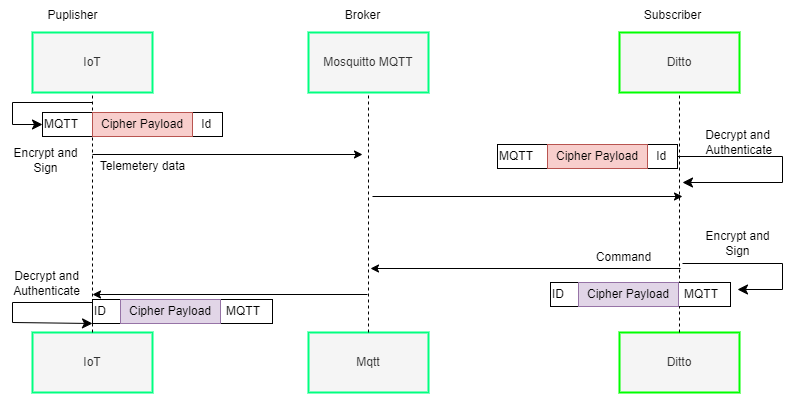
\includegraphics[width=\textwidth]{images/fp/payloadenc.drawio.png}
     \caption{Scheme of Payload Encryption With Authentication Over MQTT Protocol. }
    \label{fig:payload-encauth-schem}
\end{figure}

To achieve payload encryption using ASCON or AES-GCM algorithm over the MQTT protocol, the following steps should be taken. 
\begin{itemize}
    \item[-] \textit{Device ID registration}: Each connected device to Ditto should have a unique device ID. 
    \item[-] \textit{Generate and manage encryption keys}: The device and the Digital Twin agree on a symmetric key. 
    \item[-] \textit{Encrypting and Sending a message}: The sender encrypts the payload of the message along with a tag generated and publishes it to the MQTT broker. The associated data in this case is the unique ID of the device that is sending and receiving data to and from the Digital Twin. 
    \item[-] \textit{Forwarding or Proxing}: The MQTT broker proxies the message through the publisher-subscriber setting. 
    \item[-] \textit{Decryption and Authentication}: The receiver (subscriber) receives the MQTT message and decrypts the payload using a symmetric key retrieved using the device ID of the sender. The receiver then authenticates the payload to ensure that it is from the expected sender and that it has not been tampered with.
    
\end{itemize}

\textbf{\textit{End-To-End Payload Encryption and Authentication:}}
Our communication scheme is based on payload authenticated encryption using one of the AEAD (authenticated encryption with associated data) algorithms over the MQTT protocol. This Implicitly provides end-to-end confidentiality and integrity of a communicated message between Digital Twin and (I)IoT. The Mosquitto broker, which sits between Digital Twin and (I)IoT,  acts as a proxy for forwarding encrypted payload messages. Hence, only the communication parties are able to decrypt and authenticate the payload. 

